%!TEX root = lot2.tex

%--------------------------CARTES NEUTRE------------------------------------------------------------------------------------------------

\begin{tikzpicture} %Recto
	%Fond
    \node[anchor=south west,inner sep=0] (carte) at (0,0) {
\includegraphics[width=7.1 cm, height=9.6 cm]{fonds/noir.png}};
    \node[anchor=center] at (carte.center) {
\includegraphics[width=\cardwidth cm, height=\cardheight cm]{fonds/fond_plan.png}};
\end{tikzpicture}

\begin{tikzpicture} %Verso
	%Fond
    \node[anchor=south west,inner sep=0] (carte) at (0,0) {
\includegraphics[width=7.1 cm, height=9.6 cm]{fonds/noir.png}};
    \node[anchor=center] at (carte.center) {
\includegraphics[width=\cardwidth cm, height=\cardheight cm]{fonds/fond_plan.png}};
\end{tikzpicture}

%%%%%%%%%%%%%%%%%%%%%%%%%%%%%%%%%%%%%%%%%%NEVER MISS A DROP
\begin{tikzpicture} %Recto
	%Fond
    \node[anchor=south west,inner sep=0] (carte) at (0,0) {
\includegraphics[width=7.1 cm, height=9.6 cm]{fonds/noir.png}};
    \node[anchor=center] at (carte.center) {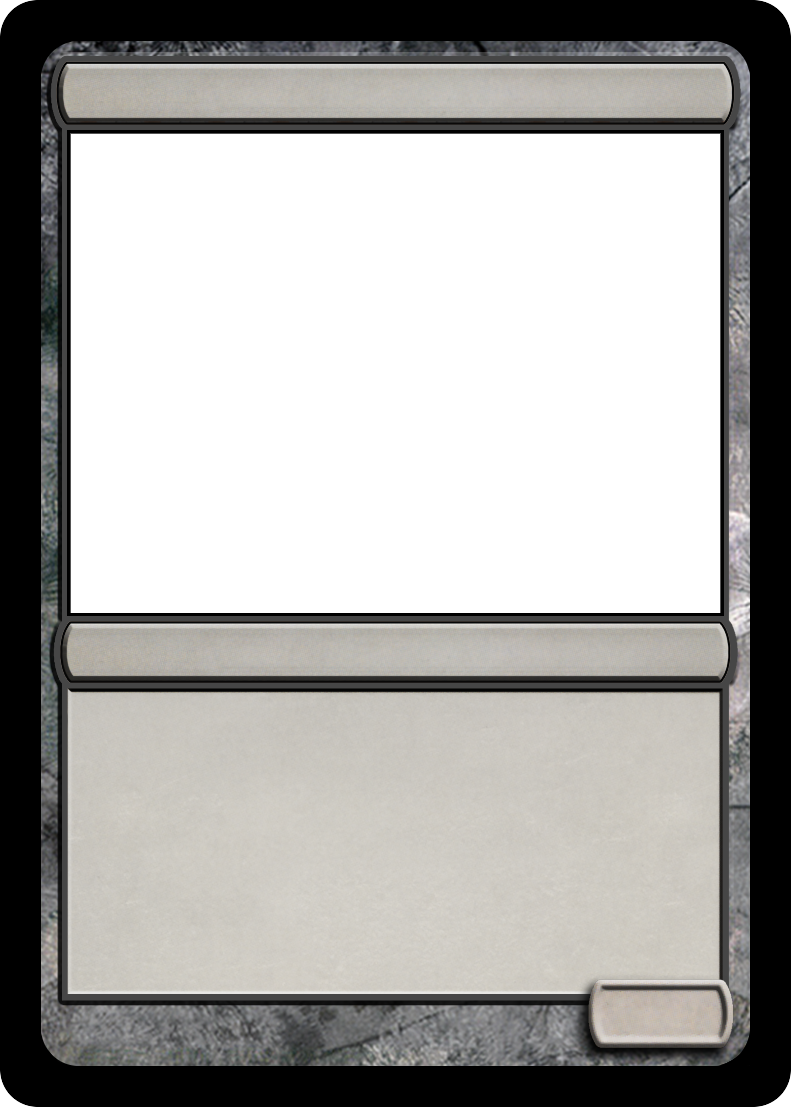
\includegraphics[width=\cardwidth cm, height=\cardheight cm]{fonds/fond_neutre.png}};

    %Titre
	\node[anchor=center] at (\titleX,\titleY) {\titlefont Never Miss A Drop !};

	%Image
	\node[anchor=center] at (\imageX,\imageY) {
\includegraphics[width=\imageWidth px, height=\imageHeight px]{images/never_miss.jpg}};
	\node[anchor=center] at (6.1,4.5) {
\includegraphics[width=12 px, height=6 px]{fonds2/legacy.jpg}};

	%Type
	\node[anchor=center] at (\typeX,\typeY) {\typefont Neutre};

	%Description
	\node[anchor=north west, text width=5.6cm] (description) at (\descriptionX,\descriptionY) {\descriptionfont\setsize{7} Grace au market piss, ne ratez plus une goutte ! Remplissez un verre d'eau à la hauteur de votre choix. Jusqu'à ce qu'un joueur déborde, chacun doit ajouter un NFT (faire couler de l'eau) dans le verre. Celui qui échoue doit piocher une carte, puis le tour se termine\par};

	%Punchline
	\node[anchor=north west, text width=5.6cm, below = 1pt of description] (punchline) {\punchlinefont\setsize{7}``Pour plus d'inclusivité, les toilettes d'entresol sont désormais agenrées.''\par};

	%Separateur !!!!!PAS TOUCHE!!!!!
	\fill[black,path fading=west] (description.south west) rectangle (punchline.north);
	\fill[black,path fading=east] (punchline.north) rectangle (description.south east);

	%Numéro !!!!!PAS TOUCHE!!!!!
	\node[anchor=center] at (\numberX,\numberY) {\numberfont \cardnumber};
\end{tikzpicture}\verso %Verso



%%%%%%%%%%%%%%%%%%%%%%%%%%%%%%%%%%%%%%%%%%HAN SOLO ROGERS
\begin{tikzpicture} %Recto
	%Fond
    \node[anchor=south west,inner sep=0] (carte) at (0,0) {
\includegraphics[width=7.1 cm, height=9.6 cm]{fonds/noir.png}};
    \node[anchor=center] at (carte.center) {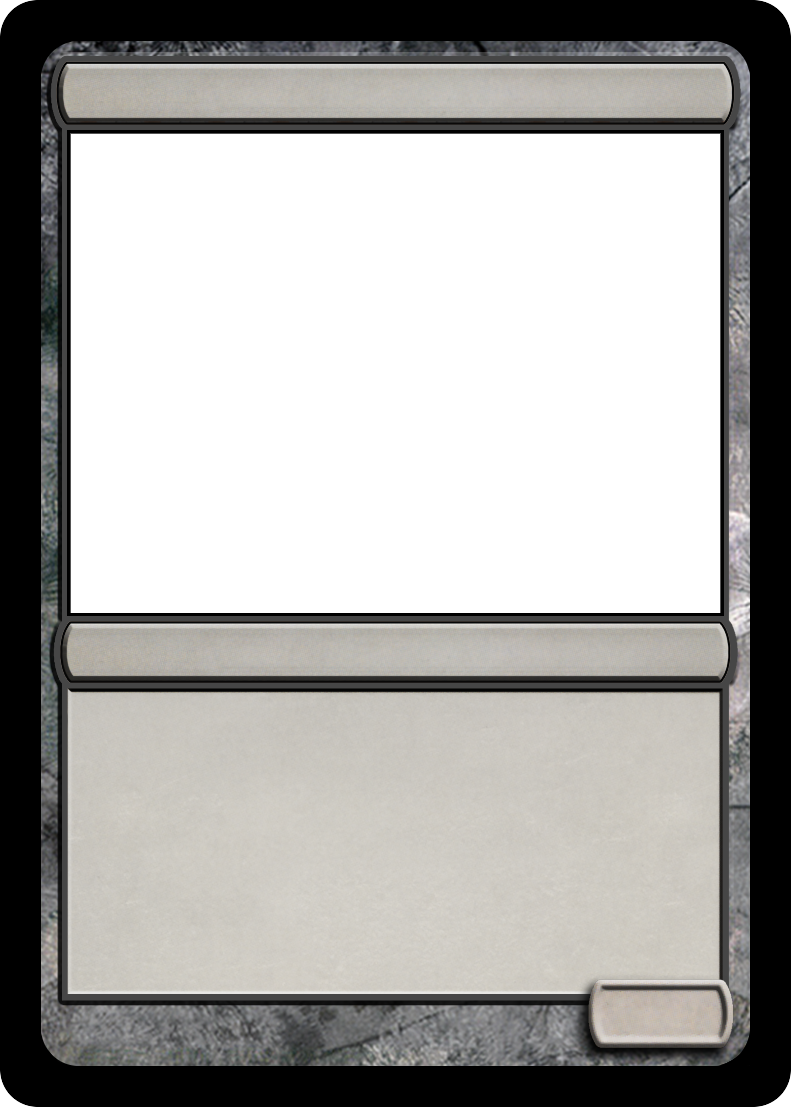
\includegraphics[width=\cardwidth cm, height=\cardheight cm]{fonds/fond_neutre.png}};

    %Titre
	\node[anchor=center] at (\titleX,\titleY) {\titlefont Han Solo Rogers};

	%Image
	\node[anchor=center] at (\imageX,\imageY) {
\includegraphics[width=\imageWidth px, height=\imageHeight px]{images/ian.jpg}};
	\node[anchor=center] at (6.1,4.5) {
\includegraphics[width=12 px, height=6 px]{fonds2/legacy.jpg}};

	%Type
	\node[anchor=center] at (\typeX,\typeY) {\typefont Neutre};

	%Description
	\node[anchor=north west, text width=5.6cm] (description) at (\descriptionX,\descriptionY) {\descriptionfont\setsize{7} Vous allez dégoter le futur artiste qui sera sponsorisé par le Market Pass ! Chaque joueur doit faire un dessin de singe. Vous choisissez le plus beau, l'auteur peut défausser une carte.\par};

	%Punchline
	\node[anchor=north west, text width=5.6cm, below = 1pt of description] (punchline) {\punchlinefont\setsize{7}``I have got a very good feeling about this.''\par};

	%Separateur !!!!!PAS TOUCHE!!!!!
	\fill[black,path fading=west] (description.south west) rectangle (punchline.north);
	\fill[black,path fading=east] (punchline.north) rectangle (description.south east);

	%Numéro !!!!!PAS TOUCHE!!!!!
	\node[anchor=center] at (\numberX,\numberY) {\numberfont \cardnumber};
\end{tikzpicture}\verso %Verso




%%%%%%%%%%%%%%%%%%%%%%%%%%%%%%%%%%%%%%%%%%SUICIDAL TENDENCIES
\begin{tikzpicture} %Recto
	%Fond
    \node[anchor=south west,inner sep=0] (carte) at (0,0) {
\includegraphics[width=7.1 cm, height=9.6 cm]{fonds/noir.png}};
    \node[anchor=center] at (carte.center) {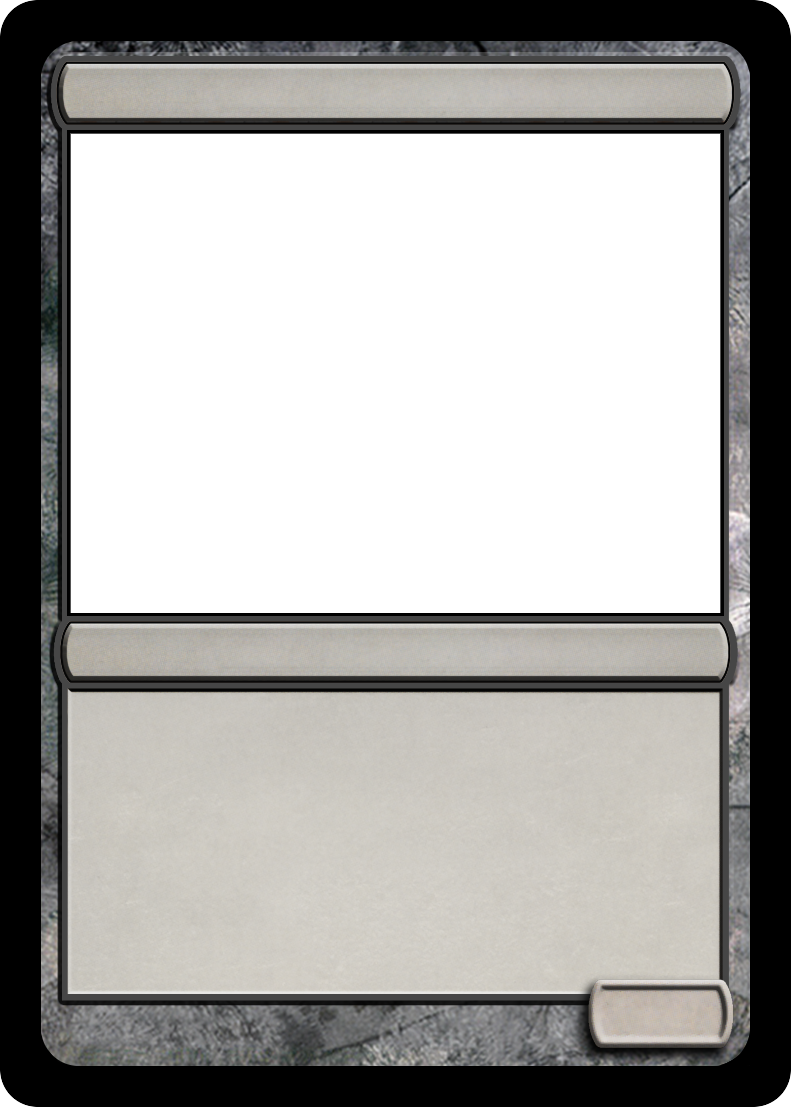
\includegraphics[width=\cardwidth cm, height=\cardheight cm]{fonds/fond_neutre.png}};

    %Titre
	\node[anchor=center] at (\titleX,\titleY) {\titlefont Suicidal Tendencies};

	%Image
	\node[anchor=center] at (\imageX,\imageY) {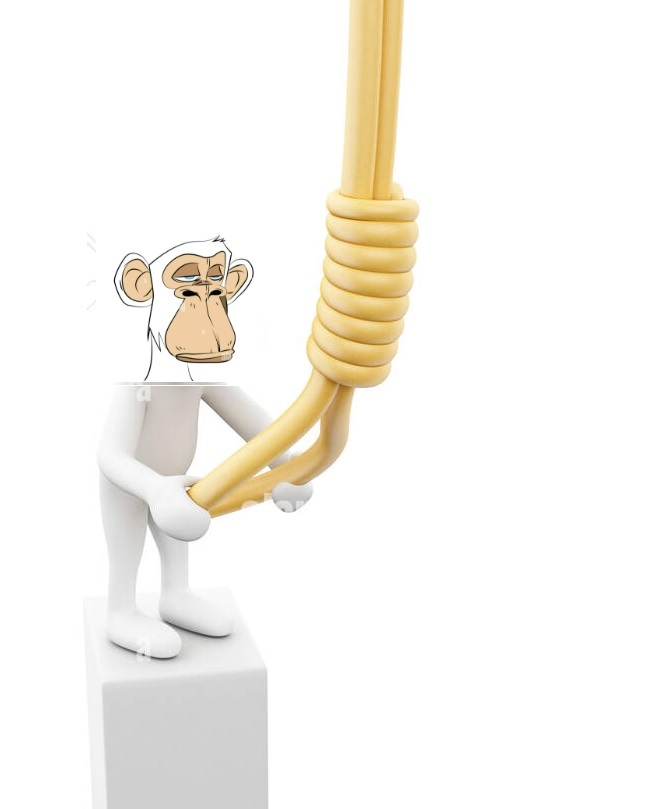
\includegraphics[width=\imageWidth px, height=\imageHeight px]{images/suicide.jpg}};
	\node[anchor=center] at (6.1,4.5) {
\includegraphics[width=12 px, height=6 px]{fonds2/legacy.jpg}};

	%Type
	\node[anchor=center] at (\typeX,\typeY) {\typefont Neutre};

	%Description
	\node[anchor=north west, text width=5.6cm] (description) at (\descriptionX,\descriptionY) {\descriptionfont\setsize{8} Cette carte peut être jouée si la carte {\emph Séminaire à Tenerife} est sur la table. Le joueur devant la carte décide subitement de confesser sa haine des NFT devant toute l'entreprise. Il crie Banzaï et pioche deux cartes.\par};

	%Punchline
	\node[anchor=north west, text width=5.6cm, below = 1pt of description] (punchline) {\punchlinefont\setsize{8}``Kevin Lombaire ne pouvait s'empècher de dire ce qu'il pensait. R.I.P. ''\par};

	%Separateur !!!!!PAS TOUCHE!!!!!
	\fill[black,path fading=west] (description.south west) rectangle (punchline.north);
	\fill[black,path fading=east] (punchline.north) rectangle (description.south east);

	%Numéro !!!!!PAS TOUCHE!!!!!
	\node[anchor=center] at (\numberX,\numberY) {\numberfont \cardnumber};
\end{tikzpicture}\verso %Verso



%%%%%%%%%%%%%%%%%%%%%%%%%%%%%%%%%%%%%%%%%%BUS
\begin{tikzpicture} %Recto
	%Fond
    \node[anchor=south west,inner sep=0] (carte) at (0,0) {
\includegraphics[width=7.1 cm, height=9.6 cm]{fonds/noir.png}};
    \node[anchor=center] at (carte.center) {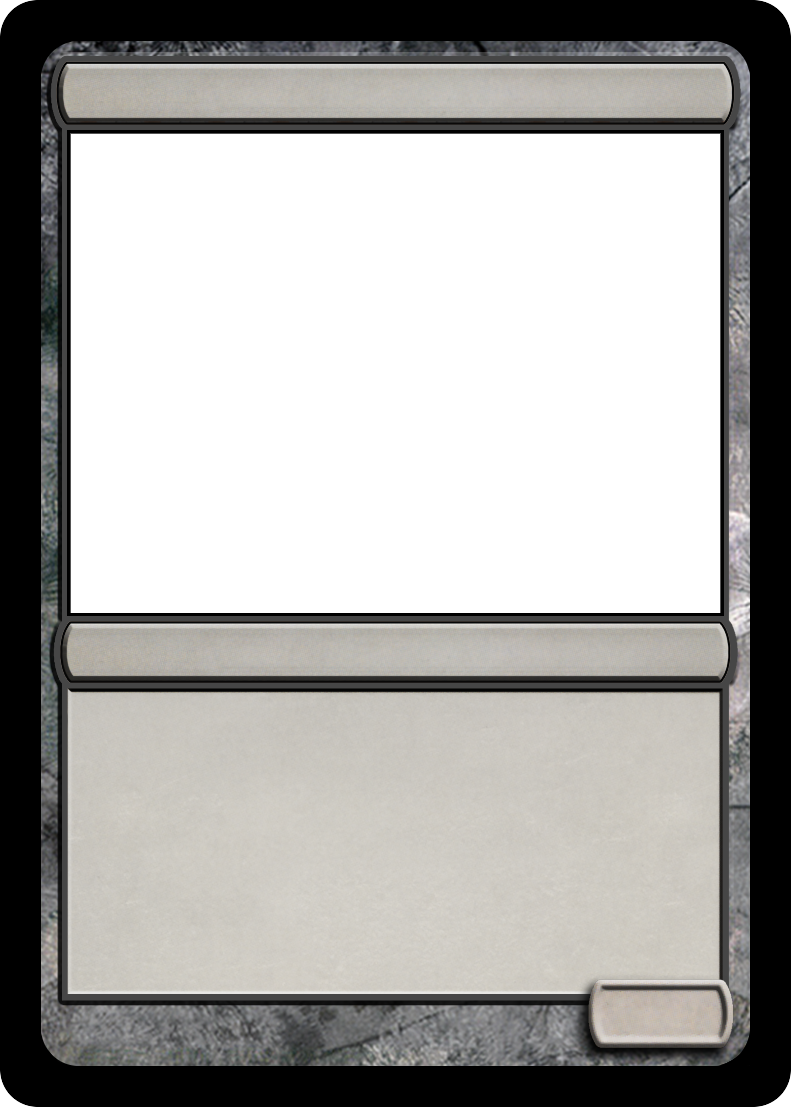
\includegraphics[width=\cardwidth cm, height=\cardheight cm]{fonds/fond_neutre.png}};

    %Titre
	\node[anchor=center] at (\titleX,\titleY) {\titlefont Bus pour Cosmos};

	%Image
	\node[anchor=center] at (\imageX,\imageY) {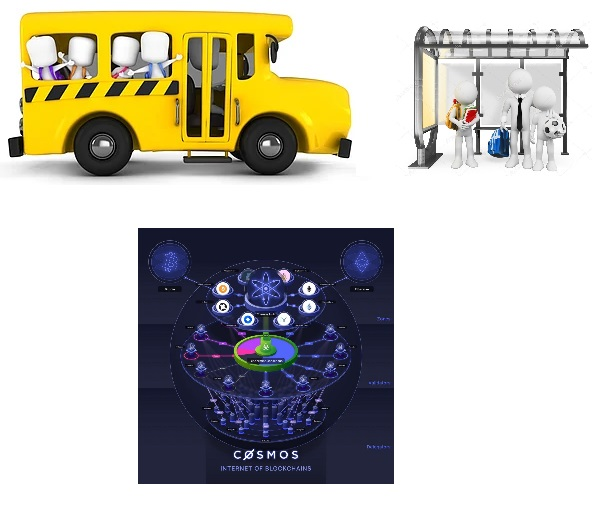
\includegraphics[width=\imageWidth px, height=\imageHeight px]{images/bus.jpg}};
	\node[anchor=center] at (6.1,4.5) {
\includegraphics[width=12 px, height=6 px]{fonds2/legacy.jpg}};

	%Type
	\node[anchor=center] at (\typeX,\typeY) {\typefont Neutre};

	%Description
	\node[anchor=north west, text width=5.6cm] (description) at (\descriptionX,\descriptionY) {\descriptionfont\setsize{8} Lorsque cette carte est jouée le stagiaire ne peut pas avoir de tour bonus car il préfère prendre le bus à la place. Ce dernier doit faire le tour de la pièce jusqu'à la fin du tour de jeu. Ben oui, c'est loin le cosmos !\par};

	%Punchline
	\node[anchor=north west, text width=5.6cm, below = 1pt of description] (punchline) {\punchlinefont\setsize{8}``Au moins Grand Corp Malade, lui il slamme. ''\par};

	%Separateur !!!!!PAS TOUCHE!!!!!
	\fill[black,path fading=west] (description.south west) rectangle (punchline.north);
	\fill[black,path fading=east] (punchline.north) rectangle (description.south east);

	%Numéro !!!!!PAS TOUCHE!!!!!
	\node[anchor=center] at (\numberX,\numberY) {\numberfont \cardnumber};
\end{tikzpicture}\verso %Verso



